
\section{\heiti 一级标题*字体为4号黑体*标题1}

这是一个CTEX的utf-8编码例子,{\kaishu 这里是楷体显示},{\songti 这里是宋体显示},{\heiti 这里是黑体显示},{\fangsong 这里是仿宋显示}。另外一种方式:\textit{这是楷体显示,but英文和数字是斜体abcABC123},\textsf{这是黑体显示abcACB123},\texttt{这是仿宋显示abcABC123}。

\subsection{\heiti 关于数学部分}
数学、中英文皆可以混排。You can intersperse math, Chinese and English (Latin script) without adding extra environments.

\subsection{\heiti 对投稿的基本要求}

(1) 研究性论文主体应包括引言(重点论述研究的科学问题、意义、解决思路、价值、贡献等)、相关工作(为与引言部分独立的一个章节)、主要成果论述、关键实现技术、验证(对比实验或理论证明)、结论(结束语)等内容;系统实现或实验应有关键点的详细论述,以便读者能够重复实现论文所述成果。实验应有具体的实验环境设置、全面细致的数据对比分析。

(2) 综述应包括引言、问题与挑战、研究现状分析、未来研究方向、结论等内容。以分析、对比为主,避免堆砌文献或一般性介绍、叙述。

(3) 定理证明、公式推导、大篇幅的数学论述、原始数据,放到论文最后的附录中。

{\bf 稿件提交时的基本要求:}

(1) 本模板中要求的各项内容正确齐全,无遗漏;

(2) 语句通顺,无中文、英文语法错误,易于阅读理解,符号使用正确,图、表清晰无误;

(3) 在学术、技术上,论文内容正确无误,各项内容确定。

{\heiti \subsection{二级标题 *字体为5号黑体*标题2}}
\subsubsection{三级标题 *字体为5号宋体*标题3}
*正文部分, 字体为5号宋体* 正文文字

\textbf{正文文字要求语句通顺,无语法错误,结构合理,条理清楚,不影响审稿人、读者阅读理解全文内容。以下几类问题请作者们特别注意}:

1) 文章题目应明确反映文章的思想和方法;文字流畅,表述清楚;

2) 中文文字、英文表达无语法错误;

3) 公式中无符号、表达式的疏漏,没有同一个符号表示两种意思的情况;

4) 数学中使用的符号、函数名用斜体;

5) 使用的量符合法定计量单位标准;

6) 矢量为黑体,标量为白体;

7) 变量或表示变化的量用斜体;

8) 图表规范,量、线、序无误,位置正确(图表必须在正文中有所表述后出现,即{\ldots}如图1所示)(注意纵、横坐标应有坐标名称和刻度值)。

9) 列出的参考文献必须在文中按顺序引用,即参考文献顺序与引用顺序一致,各项信息齐全(格式见参考文献部分);

10) 首次出现的缩写需写明全称,首次出现的符号需作出解释。

11) 图的图例说明、坐标说明全部用中文或量符号。

\textbf{12) 图应为矢量图。}

13) 表中表头文字采用中文。

14) 公式尺寸:

标准:10.5磅

下标/上标:5.8磅

次下标/上标:4.5磅

符号:16磅

次符号:10.5磅

15) 组合单位采用标准格式,如:``pJ/bit/m$^{4}$''应为 ``pJ/(bit$\cdot
$m$^{4})$''

\textbf{定理1}.\quad ******. *定理内容.*

[``定义''、``假设''、``公理''、``引理''等的排版格式与此相同,详细定理证明、公式可放在附录中]

\texttt{证明}.\quad  *证明过程.* [``例 x''等的排版格式相同]

\rightline {证毕.}

\begin{figure}[H]
\centerline{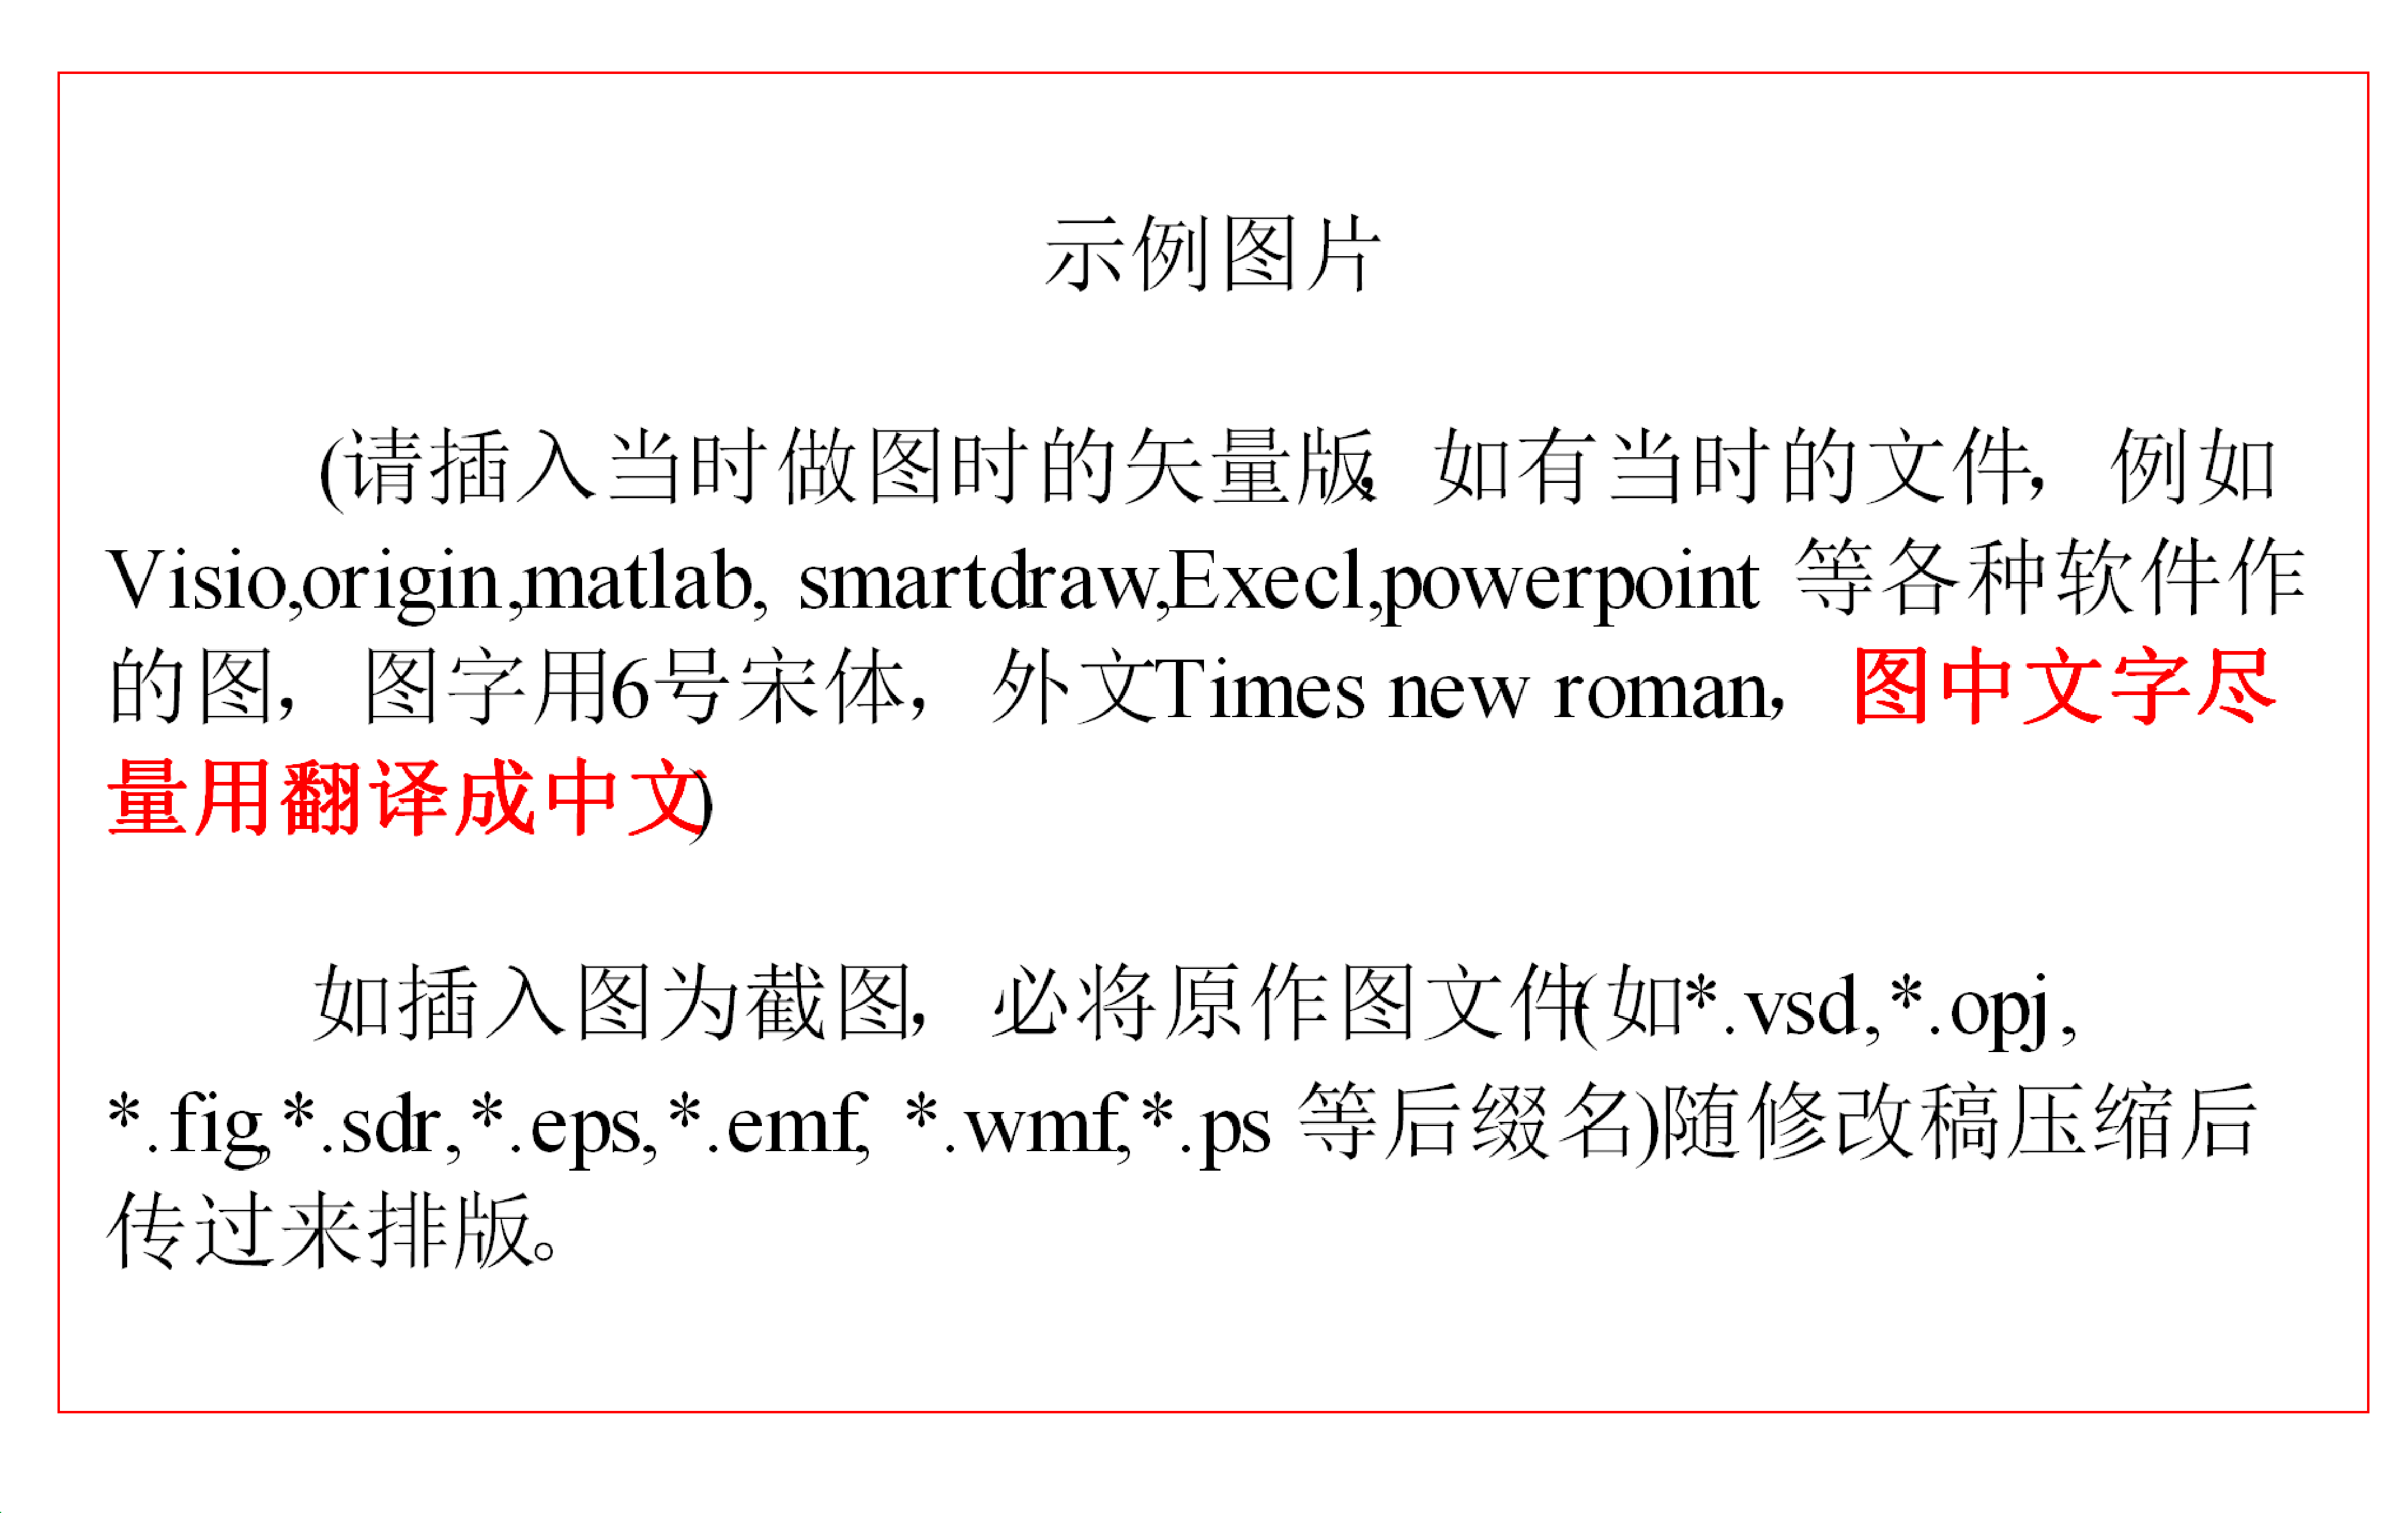
\includegraphics[width=3.15in,height=1.98in]{CJC1.pdf}}
{\zihao{5}图X\quad  图片说明 *字体为小5号,图片应为黑白图,图中的子图要有子图说明*}
\label{fig1}
\end{figure}

\begin{table}[H]
\centering {\heiti 表X\quad 表说明 *表说明采用黑体*}
% \caption{表说明 *表说明采用黑体*}
\vspace {-2.5mm}
\begin{center}
\begin{tabular}{ll}
\toprule
*示例表格*&*第1行为表头,表头要有内容* \\
\hline
&
 \\
&
 \\
&
 \\
&
 \\
\bottomrule
\end{tabular}
\label{tab1}
\end{center}
\end{table}

{\heiti 过程X}.\quad 过程名称

{\zihao{5-}*《计算机学报》的方法过程描述字体为小5号宋体,IF、THEN等伪代码关键词全部用大写字母,变量和函数名称用斜体*}


{\heiti 算法\textbf{Y}}.\quad 算法名称.
{\zihao{5-}

\noindent 输入:{\ldots} {\ldots}

\noindent 输出:{\ldots} {\ldots}

*《计算机学报》的算法描述字体为小5号宋体, IF、THEN等伪代码关键词全部用大写字母,变量和函数名称用斜体*}